\documentclass[%
    thesis=ma, %
    language=american, %
    paper=a4,%
    listings,
    online,
    %draft,
    final,
]{isw}

\listfiles


\setcounter{errorcontextlines}{999}

\title{This shall be a great thesis paper with an extremely long title but who cares}
\subtitle{Some theses even have subtitles}
\author{Philipp Tempel}
\major{Technische Kybernetik}
\examiner{Jun.-Prof.~Dr.-Ing.~Andreas Pott}
\major{Technische Kybernetik}
\supervisor{Dipl.-Ing.~Philipp Tempel}
%\matriculation{2411697}

\usepackage{lipsum}

\begin{document}
    \maketitle
    
    \begin{otherlanguage}{ngerman}\maketitle \end{otherlanguage}
    
    \tableofcontents
    
    \listoffigures
    
    \listoftables
    
    \listoftodos
    
    \chapter[The Short Title of the Chapter Showing Up in the TOC and the Page Headers]{The Very First Chapter With a Very Long Title Just to See What it Looks Like Since it Spans Multiple Lines in the ToC}
    
    \chapter{A Second Chapter}
    
    \section{A First Section}
    
    \subsection{A Sample Subsection}
    
    \subsubsection{A Sample Subsubsection}
    
    \paragraph{A Sample Paragraph}
    
    \subparagraph{A Sample Subparagraph}
    
    \begin{figure}
        \centering
        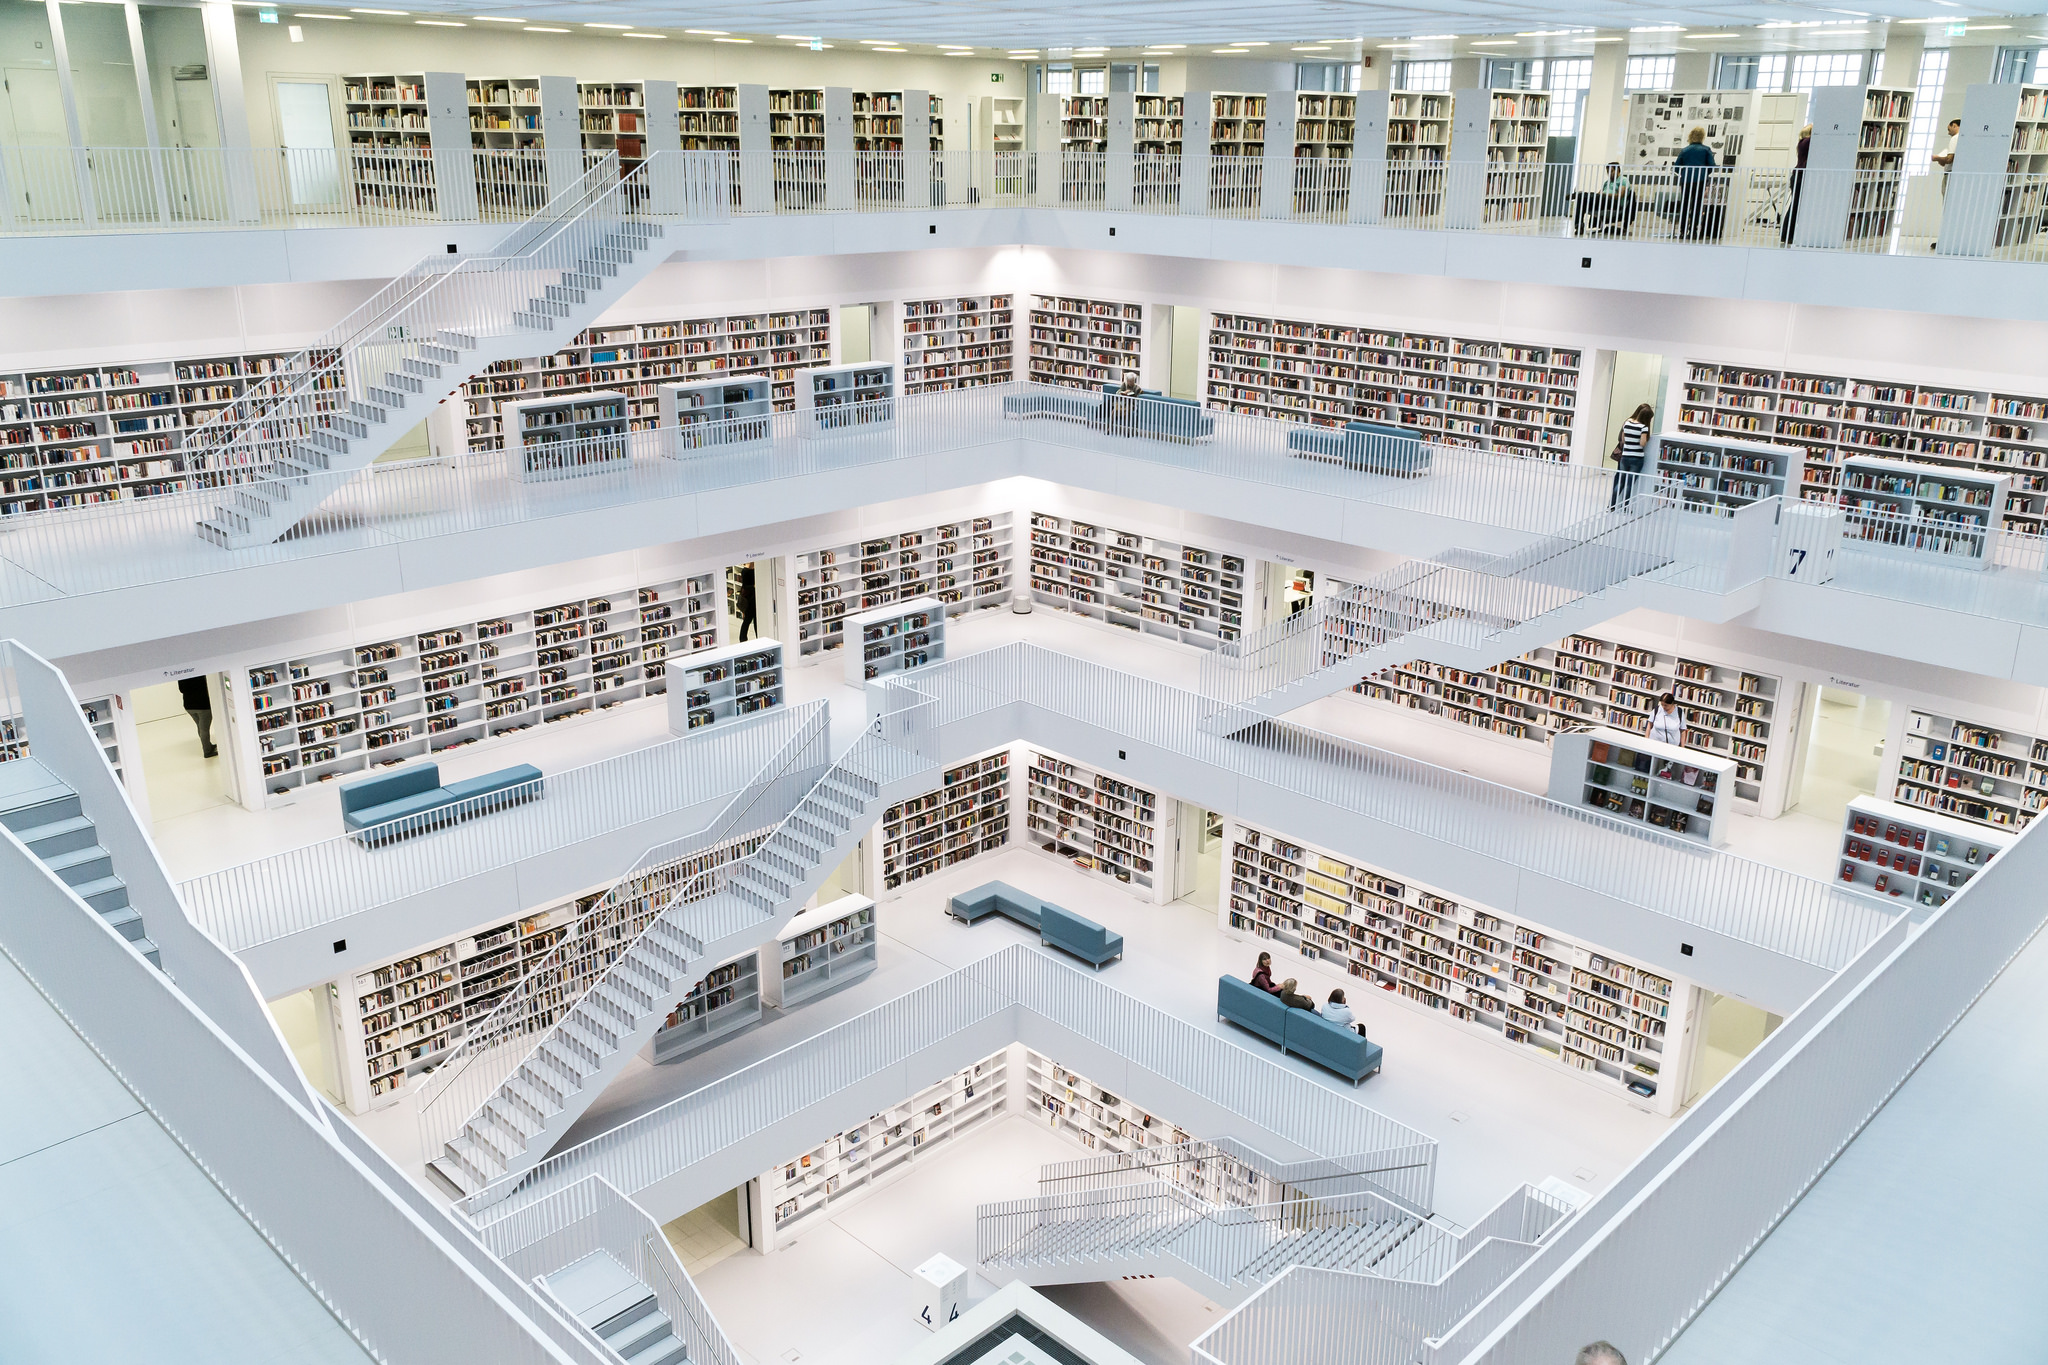
\includegraphics[width=\linewidth, keepaspectratio=true]{placeholder/14942249547_f7f1d3e8bd_k}
        \caption{A sample figure to show the effect of a loooong looooong caption. Credits by \url{https://www.flickr.com/photos/schubi74/14942249547/}.}
        \label{fig:sample-figure}
    \end{figure}
    
%    \begin{listing}
%        \begin{minted}{latex}
%\begin{figure}
%    \centering
%    \includegraphics[width=\linewidth, keepaspectratio=true]%
%        {placeholder/14942249547_f7f1d3e8bd_k}
%    \caption{A sample figure to show the effect of a loooong looooong caption. %
%        Credits by \url{https://www.flickr.com/photos/schubi74/14942249547/}.}
%    \label{fig:sample-figure}
%\end{figure}
%        \end{minted}
%        \caption{Sample code for \cref{fig:sample-figure}}
%        \label{lst:sample-code}
%    \end{listing}
    
    For figures the guidelines are:
    \begin{itemize}
        \item Always center images using \verb|\centering| as the very first command of the \verb|figure|-environment.
        \item Make sure to set the width of your included images explicitely using the \verb|width=\linewidth| option.
        \item Don't forget to keep the aspect ratio of images if you change their width.
        \item Never ever under sample images. In other words: never ever enlarge images.
        \item It's best to use vector graphics i.e., \verb|*.eps| or \verb|*.tikz| for proper quality in both PDFs as well as on screen.
        \item Add a caption to your image. Captions must be below the image.
        \item Let the labels be handled automatically by \LaTeX. A best practice is to set the prefix of figures' labels to \verb|fig:|.
        \item For a good example see \cref{fig:sample-figure} and its code at \cref{lst:sample-code} (this reference was created using the \verb|\cref{}| command).
        \item Always add a full stop to your figure captions like so.
    \end{itemize}
    
    
    \section{Referencing}
    
    Referencing may be done using \verb|\ref{label}| even though usage of \verb|\cref{label}| is encouraged for that it automatically typesets the appropriate type like \texttt{Eqn.} or \texttt{Fig.}, \texttt{Tbl.}, or \texttt{Listing} to whatever is being reference. At the beginning of a sentence \verb|\Cref{label}| must be used to fully the referenced type in words. \Cref{fig:sample-figure} refers to a sample figure at the beginning of a sentence, while \cref{fig:sample-figure} refers to a sample figure in text.
    
    \begin{itemize}
        \item Capitalise and write in words the reference object at the beginning of a sentence
        \item Otherwise use the abbreviated forms of \texttt{Fig.}, \texttt{Eqn.}, and \texttt{Tbl.} for referencing figures, equations, and tables, respectively
        \item Refer to the \verb|cleveref| package documentation at \url {http://www.ctan.org/pkg/cleveref}
    \end{itemize}
    
\end{document}